\documentclass[12pt]{book}
\usepackage[margin=.85in]{geometry} % for MARGIN
\usepackage[many]{tcolorbox}    	% for COLORED BOXES (tikz and xcolor included)


\usepackage{multicol}   
\usepackage{enumerate}
\usepackage[shortlabels]{enumitem}
\usepackage{varwidth}
\usepackage{tasks}
\usepackage[export]{adjustbox}

\usepackage{titleps}
\usepackage{setspace}               % for LINE SPACING
\usepackage[⟨options⟩]{fancyhdr}
\usepackage{enumitem}
\setlist{nosep}
\usepackage{tikz}
\usepackage{pgfplots}
\pgfplotsset{compat=1.5.1}
\usetikzlibrary{datavisualization}
\usetikzlibrary{datavisualization.formats.functions}

\newcommand{\D}{\displaystyle}


\setlength\parindent{0pt}   % killing indentation for all the text
\setstretch{1.3}            % setting line spacing to 1.3
\setlength\columnsep{0.25in} % setting length of column separator
\pagestyle{fancy}           % setting pagestyle to be headings

\usepackage[]{titlesec}

\fancyhead[L]{Math V04 - College Algebra}
\fancyhead[R]{Christina Papazacharioudakis}

\tcbset{
    sharp corners,
    colback = white,
    before skip = 0.2cm,    % add extra space before the box
    after skip = 0.5cm      % add extra space after the box
}                           % setting global options for tcolorbox

    \newtcolorbox{boxR}{
    fontupper = \color{black}, % font color
    boxrule = 1.5pt,
    colframe = black,
    rounded corners,
    arc = 5pt   % corners roundness
}

\definecolor{ballblue}{rgb}{0.13, 0.67, 0.8}

\begin{document}


{\Large \textbf{2.7 Linear Inequalities and Absolute Value Inequalities}}

\vspace{3mm}

In this section, we start to look at solving inequalities. When we solve inequalities, we usually get that $x$ can take on a range of values. So we first need to establish how we handle $x$ taking on multiple values using \textbf{interval notation}.

\vspace{3mm}
{\large \textbf{Using Interval Notation}}
\vspace{3mm}

Let's say we want to make sense of $x \geq 4$ (``$x$ is greater than or equal to four"). We can see this in a few different ways. 

The first method is to use a number line:
\vspace{3mm}

\centerline{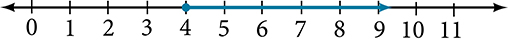
\includegraphics[height=10mm, width=110mm]{numberline.jpeg}}
The blue ray starts at $x=4$ with a closed circle since we include $4$, and continues to infinity on the right of 4, indicated by the arrow.
\vspace{3mm}

The second method is to use set-builder notation: $$\{x \mid x\geq 4 \}$$ which translates to ``all real numbers $x$ such that $x$ is greater than or equal to $4$." We use brackets to represent a set. The conditions on $x$ are given after the bar symbol. 
\vspace{3mm}

The third method is \textbf{interval notation} which uses parenthesis and brackets:  $$ [4, \infty)$$

Since we include $4$, we use a bracket. Since we are looking at all possible values greater than $x$, we use infinity. Since we can't ever equal infinity, we use parenthesis there. 

\emph{Interval notation is the most useful method as it will be applied to later concepts in this course and to other higher-level math courses.}

\vspace{3mm}
Let's look at some examples using interval notation. We will use a number line as our guide (visuals can be a great guide!) 
\newpage
\underline{\textbf{Example 1 - Use Interval Notation for Numbers Greater than or Equal to $\mathbf{a}$}}
\vspace{1mm}

Use interval notation to indicate the following:
\begin{enumerate}[(a)]
    \item All real numbers that are greater than or equal to $-2$.
    \vspace{25mm}
    \item All real numbers that are between and including $-3$ and $5$
    \vspace{25mm}
\end{enumerate}

\underline{\textbf{Example 2 - Use Interval Notation for Numbers Less Than/Greater Than or Equal to $\textbf{a}$}}
\vspace{1mm}
Use interval notation to express the following:
\begin{enumerate}[(a)]
    \item All real numbers that are less than or equal to $-1$ or are greater than or equal to $1$.
    \vspace{25mm}
    \item All real numbers that are less than but not including $-2$ or greater than or equal to $3$.
      \vspace{25mm}  
\end{enumerate}



\centerline{\textbf{Table of Possible Sets}}
\vspace{3mm}

{\hspace{-14mm}
\begin{tabular}{ |l|c|c| } 
 \hline
 \textbf{Set Indicated} & \textbf{Interval Notation} & \textbf{Set-Builder Notation} \\ 
 \hline
 All real numbers between $a$ and $b$, but not including a or b & $(a,b)$ & $\{x \mid a < x < b\}$ \\ 
 \hline
 All real numbers greater than $a$, but not including $a$ & $(a,\infty)$ & $\{x \mid x > a\}$ \\ 
 \hline
 All real numbers less than $b$, but not including $b$ & $(\infty, b)$ & $\{x \mid x< b \}$ \\
 \hline
 All real numbers greater than $a$, including $a$ & $[a, \infty)$ & $\{x \mid x \geq a \}$ \\
 \hline
 All real numbers less than $b$, including $b$ & $(\infty, b ]$ & $\{x \mid x \leq b\}$ \\
 \hline
 All real numbers between $a$ and $b$, including $a$ & $[a,b)$ & $\{x \mid a \leq x < b\}$ \\
 \hline
 All real numbers between $a$ and $b$, including $b$ & $(a,b]$ & $\{x \mid a < x \leq b\}$ \\
 \hline
 All real numbers between a and b, including $a$ and $b$ & $[a,b]$ & $\{x \mid a \leq x \leq b \}$ \\
 \hline
 All real numbers less than $a$ or greater than $b$ & $(-\infty, a) \cup (b, \infty)$ & $\{ x \mid a < x \text{ or } x >b\}$ \\
 \hline
\end{tabular}
}

\newpage
{\large \textbf{Using Properties of Inequalities}}
\vspace{3mm}

When we work with solving inequalities, we can treat them similarly, but not exactly, as we treat equalities. We can use the addition property and the multiplication property to help us solve them. The one exception is when we multiply or divide by a negative number; doing so reverses the inequality symbol.
  
\begin{boxR}
    \textbf{Properties of Inequalities}
     \vspace{1mm}
    \hline
    \vspace{2mm}
    \textbf{Addition Property}: 
    $$\text{If } a < b, \text{ then } a + c < b+c$$
    \textbf{Subtraction Property}:
    $$ \text{If } a < b, \text{ then } a - c < b - c$$
    \textbf{Multiplication Property}:
    \vspace{-5mm}
    \begin{align*}
         \text{Assume } c >0. \text{ If } a < b, \text{ then } ac < bc \\ 
         \text{Assume } c <0.  \text{ If } a < b, \text{ then } ac > bc
    \end{align*}
     \textbf{Division Property ($\mathbf{c\neq 0}$)}:
    \vspace{-5mm}
    \begin{align*}
         \text{Assume } c >0. \text{ If } a < b, \text{ then } \frac{a}{c} < \frac{b}{c} \\ 
         \text{Assume } c <0.  \text{ If } a < b, \text{ then } \frac{a}{c} > \frac{b}{c}
    \end{align*}
    These also work for $a \leq b$, $a >b$, and $a \geq b$.
\end{boxR}
\underline{\textbf{Example 3 - Demonstrating the Addition and Subtraction Property}}

Solve the linear inequalities using the addition or subtraction property. State your answer in interval notation.
\begin{enumerate}[(a)]
    \item $x-15 < 4$
    \vspace{16mm}
    \item $6 \geq x-1$
    \vspace{16mm}
    \item $x+7 > 9$
    \vspace{16mm}
\end{enumerate}
\newpage

\underline{\textbf{Example 4 - Demonstrating the Multiplication and Division Property}}

Solve the linear inequalities using the multiplication and division property. State your answer in interval notation.
\begin{enumerate}[(a)]
    \item $3x< 6$
    \vspace{18mm}
    \item $ -2x-1 \geq 5$ 
    \vspace{18mm}
    \item $5-x > 10$
    \vspace{18mm}
\end{enumerate}

{\large \textbf{Solving Inequalities in One Variable Algebraically}}
\vspace{3mm}

Just like we saw before, we can perform operations on both sides of an inequality just like we have done with equations. We can also do this to combine like terms and isolate a variable.
\vspace{3mm}

\underline{\textbf{Example 5 - Solving a Linear Inequality Algebraically}}

Solve the inequality $13-7x \geq 10x-4$. State the answer in interval notation.
\vspace{40mm}

\underline{\textbf{Example 6 - Solving a Linear Inequality with Fractions}}

Solve the following inequality and write the answer in interval notation: $-\frac{3}{4}x \geq -\frac{5}{8}+ \frac{2}{3}x$
\vspace{30mm}

\newpage

{\large \textbf{Understanding Compound Inequalities}}
\vspace{3mm}

A \textbf{compound inequality} includes two inequalities in one statement. For example, $$4 < x \leq 6$$ is a compound inequality. It means that $4 < x$ and $x \leq 6$. There are two methods to solving compound inequalities. 

\begin{boxR}
    \textbf{How To}
    \vspace{1mm}
    \hline
    \vspace{2mm}
    \textbf{Given a compound inequality, solve it.}
    \begin{enumerate}
    \item Separate the compound inequality into two separate inequalities, and then perform operations on both sides.
    
    \vspace{2mm}
    \centerline{\textbf{OR}}
    \vspace{2mm}
    \item Keep the compound inequality intact, and perform operations on all three parts at the same time. 
\end{enumerate}
    
\end{boxR}
Let's look at both methods with an example. 
\vspace{3mm}

\underline{\textbf{Example 7 - Solving a Compound Inequality}}

Solve the compound inequality $3 \leq 2x+2 \leq 6$. State your answer in interval notation.


\newpage
In Example 7, we were able to leave the compound inequality in tact because $x$ was presented to us in the middle of the compound inequality. If $x$ is presented to us on more than one side, most times we cannot get $x$ by itself in the middle. In these situations, we need to look at two separate inequalities (method 1). 

\vspace{3mm}
\underline{\textbf{Example 8 - Solving a Compound Inequality with the Variable in All Three Parts}}

Solve the compound inequality with variables in all three parts: $ 5x-10 < 7x-2  < 3 + x$.
\vspace{50mm}

{\large \textbf{Solving Absolute Value Inequalities}}
\vspace{3mm} 

From the previous section, we know that the absolute value of a quantity is either positive or zero.  This section solves absolute value inequalities, which interprets an absolute value as the distance from one point to another. 

For example, lets look at solving $|x-7|=3$, $|x+5|=1$, and $|x|=2$ using a number line: 



\vspace{95mm}
We now extend this idea to inequalities.
\newpage

\begin{boxR}
    \textbf{Absolute Value Inequalities}
    \vspace{1mm}
    \hline
    \vspace{2mm}
    For an algebraic expression $X$, and $k>0$, an \textbf{absolute value inequality} is an inequality of one of the forms.
    \begin{align*}
        &|X| \leq k \text{ is equivalent to } -k < X < k \\
        &|X| \geq k \text{ is equivalent to } X < -k \text{ or } X > k 
    \end{align*} 
\end{boxR}
\vspace{3mm}
Let's look on a number line to see what this means: 
\vspace{60mm}

\underline{\textbf{Example 9 - Determining a Number within a Prescribed Distance}}

Describe all values of $x$ within a distance of $4$ from the number $5$. Express this set in interval notation.
\vspace{10mm}

Visually: 
\vspace{40mm}

Algebraically:
\newpage

\underline{\textbf{Example 10 - Solving an Absolute Value Inequality}}

Solve $|x-1| \leq 3$. State your answer in interval notation.
\end{document}